\newpage
\chapter {Specifica della soluzione Realizzata}

Di seguito verrà fornita una descrizione dell'architettura del progetto realizzato, e in particolare verrà descritto come le soluzioni progettate sono state realizzate nella pratica.

\section{Simulazione}

	\begin{figure}[htbp]
		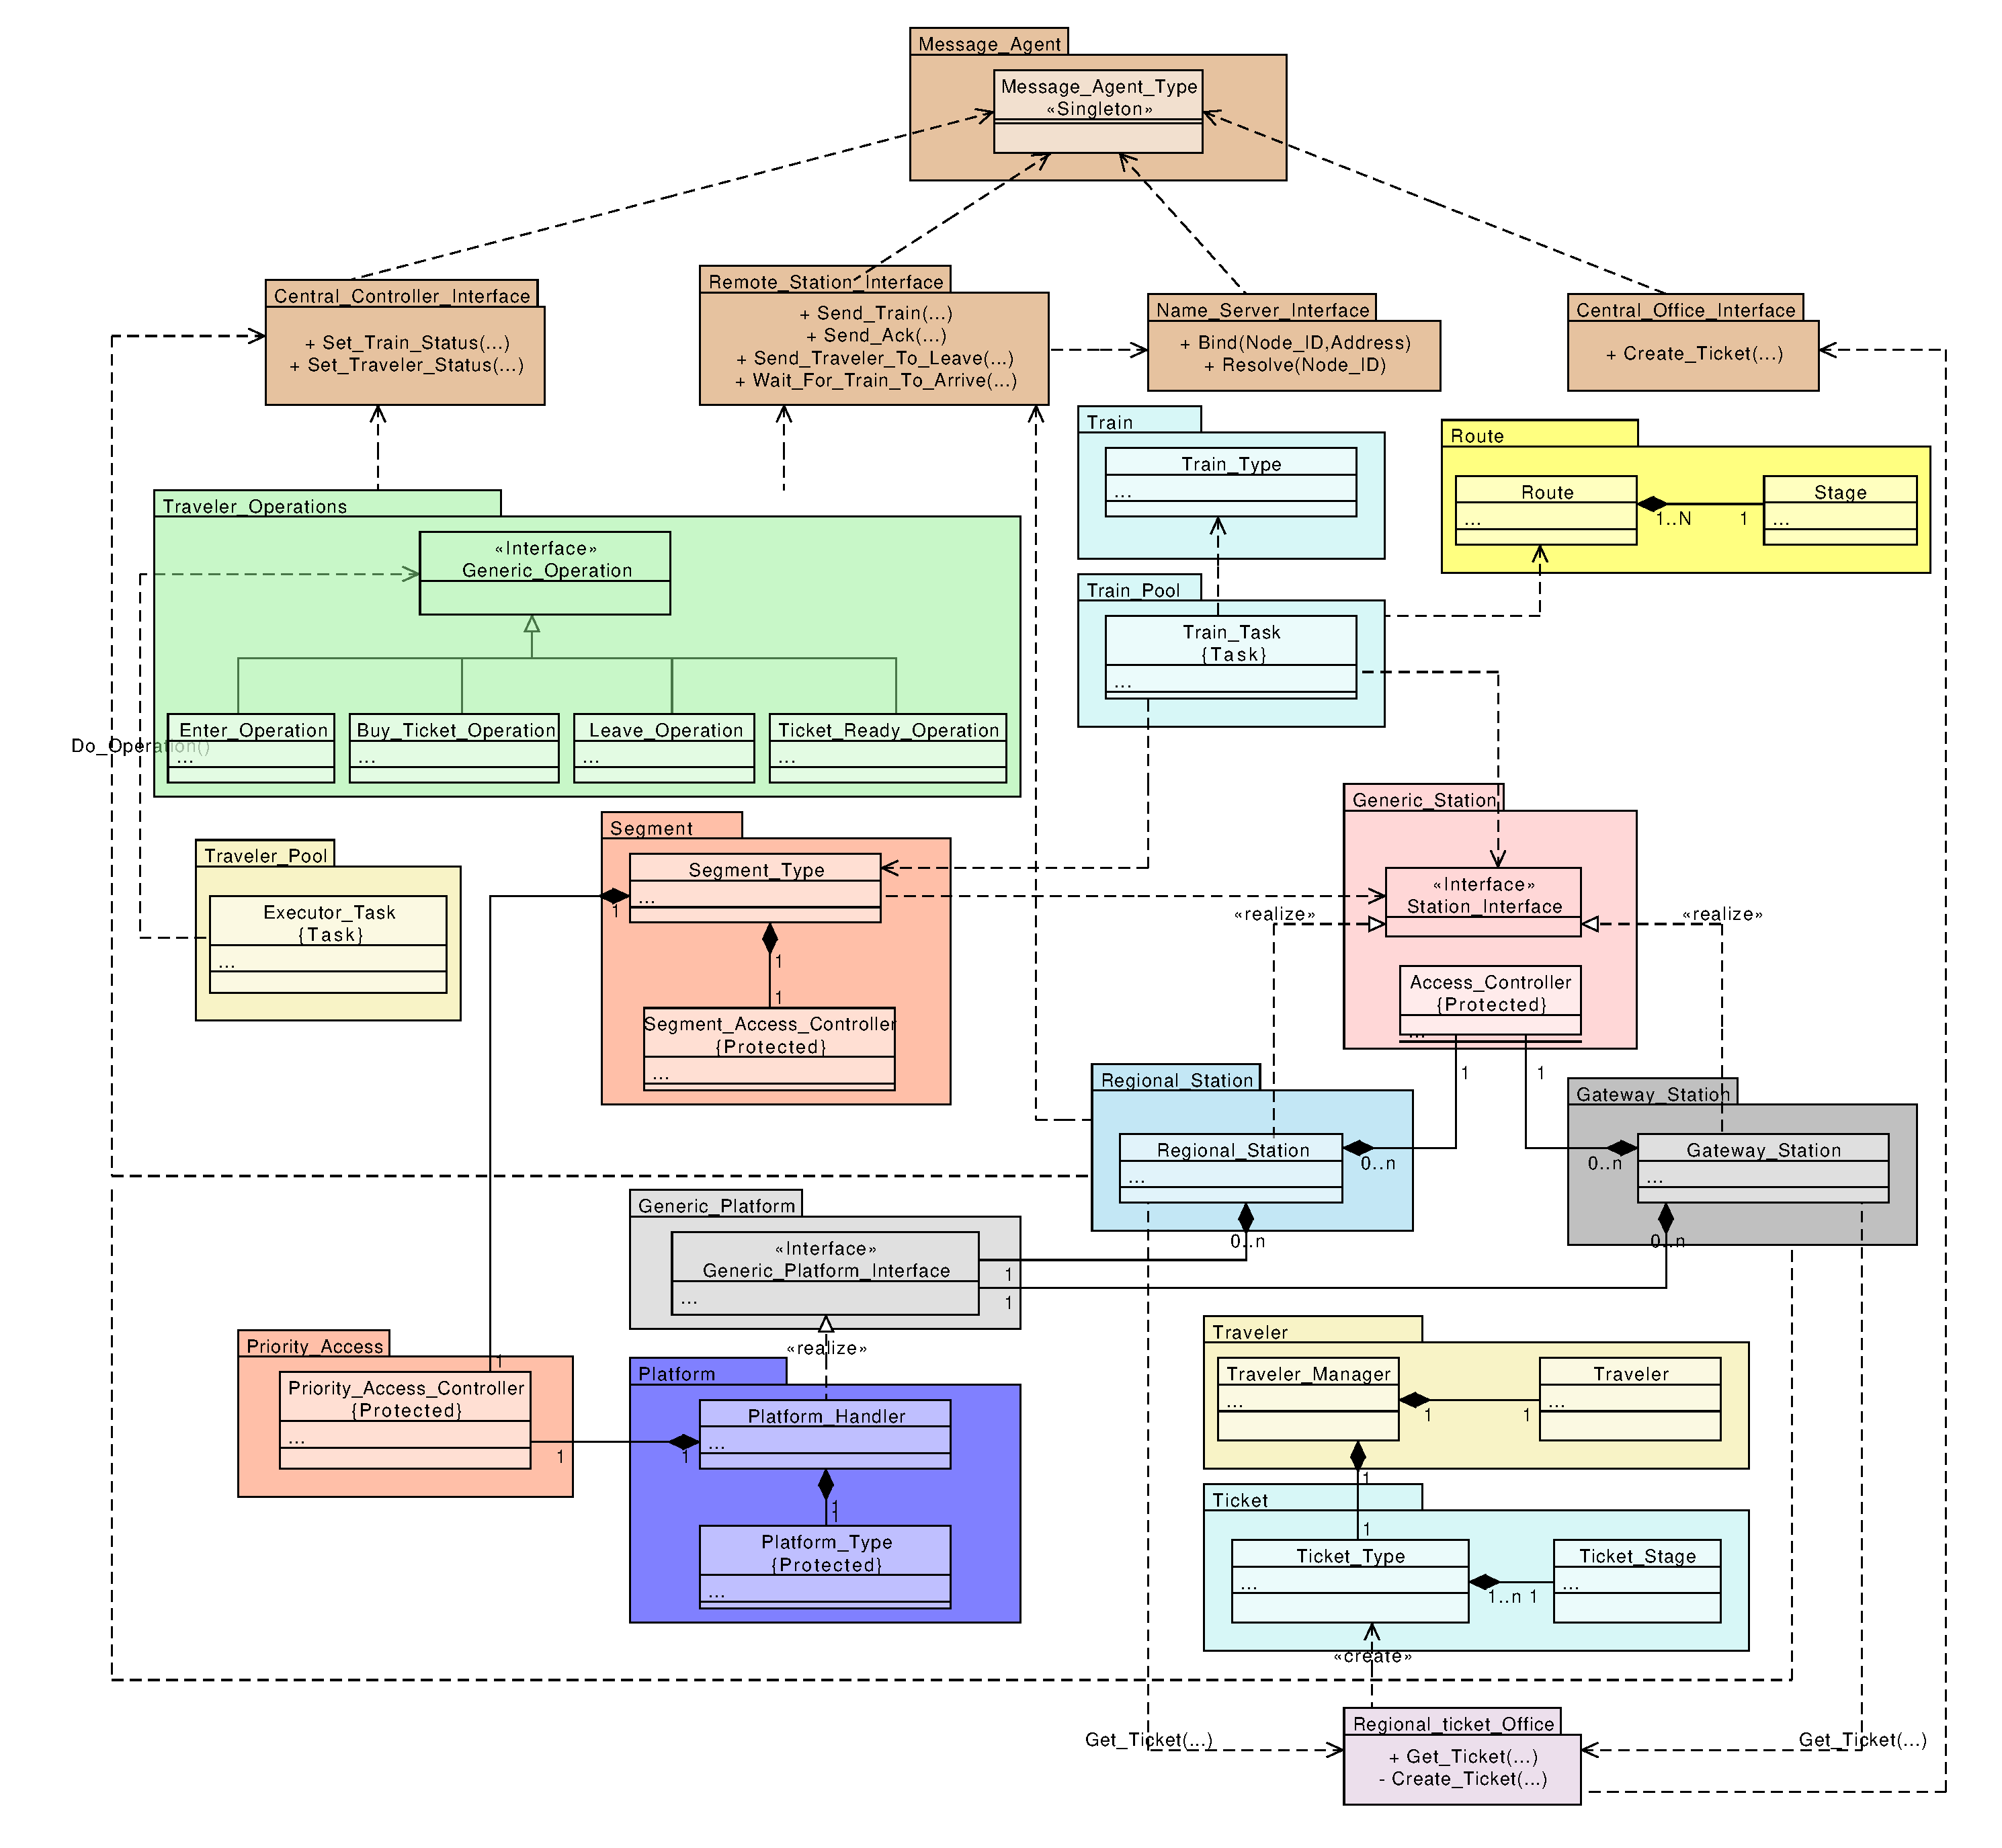
\includegraphics[scale=0.39,trim= 100mm 0mm 0mm 0mm]{imgs/Simplified_Class_Diagram.pdf}
		\caption{\footnotesize{Diagramma delle classi che illustra le componenti e le relazioni più significative che coinvolgono la simulazione.}}
		\label{img:class_diagram}
	\end{figure}

L'architettura di massima adottata per la realizzazione del core di simulazione, è visibile nel diagramma delle classi in figura \ref{img:class_diagram} nel quale, per brevità, sono stati riportati solo le informazioni più significative.
	Viene ora fornita una breve descrizione delle varie componenti che sono state utilizzate, procedendo per Package. Nelle sezioni seguenti si utilizzeranno le nozioni di \ii{Task} e \ii{Tipo protetto} definite dal linguaggio \ii{Ada}, utilizzato per l'implementazione, e verrà mostrato come le soluzioni presentate nel capitolo precedente sono state tradotte con strumenti di linguaggio.

	\subsection{Message\_Agent}
	
	Il package \ttt{Message\_Agent} fornisce un'interfaccia per l'invio di messaggi remoti. Esso contiene una classe singleton \ttt{Message\_Agent\_Type}, la quale possiede i seguenti campi dato:
	\begin{description}
		\item \ttt{- Client\_Agent : YAMI.Agents.Agent\_Access} \\
		Campo dati privato di tipo \ttt{YAMI.Agents.Agent\_Access} che contiene una istanza di Agente fornito dalla libreria \ii{Yami4}, e che viene utilizzato per l'invio e la ricezione di messaggi remoti.
		\item \ttt{- Handlers\_Map : Map} \\
		Hash-map privata, la quale associa a chiavi di tipo \ttt{String}, valori di tipo \ii{riferimento a procedura}; essa viene utilizzata per associare a ciascun servizio offerto dall'oggetto \ttt{Client\_Agent} un handler per la sua gestione.
	\end{description}
	
	Essa offre inoltre i seguenti metodi:
	
	\begin{description}
		\item \ttt{+ Listen\_To(Server\_Address)} \\
		Indica all'oggetto \ttt{Client\_Agent} di rimanere in ascolto presso l'indirizzo \ttt{Server\_Address}, attraverso il quale riceverà tutti i messaggi destinati al nodo. Nella fase di registrazione dell'oggetto remoto, viene definito un handler per la ricezione dei messaggi, il quale effettua il dispatching di ciascun messaggio ricevuto invocando la procedura corrispondente al servizio richiesto, definita nella mappa \ttt{Handlers\_Map}.
		
		\item \ttt{+ Close()} \\
		Chiude la connessione dell'oggetto \ttt{Client\_Agent}.
		
		\item \ttt{+ Send\_Message(\\
			Destination\_Address:String,\\
			Object:String,\\
			Service:String,\\
			Params:YAMI.Parameters.Parameters\_Collection,\\
			Callback)}\\
		Invia un messaggio all'oggetto remoto indicato da \ttt{Object} all'indirizzo \ttt{Destination\_Address}, richiedendo il servizio \ttt{Service}, e con i parametri indicati da \ttt{Params}. Se non nulla, la funzione di callback \ttt{Callback} viene invocata alla ricezione del messaggio di risposta, altrimenti quest'ultimo viene ignorato.
		
		\item \ttt{+ Send\_One\_Way(\\
			Destination\_Address : String,\\
			Object 				: String,\\
			Service 			: String,\\
			Params 				: YAMI.Parameters.Parameters\_Collection)}\\
		Metodo simile a \ttt{Send\_Message}, solo che non rimane in attesa della risposta al messaggio inviato.
	\end{description}
	
	Nessun meccanismo di serializzazione delle richieste è stato adottato, in quanto esso è già operato dagli oggetti della libreria \ii{Yami4}.
	
	\subsection{Central\_Controller\_Interface}
	
	Il package \ttt{Central\_Controller\_Interface} fornisce un'interfaccia per permettere alle entità della simulazione di inviare un evento di notifica alla componente remota di Controllo Centrale. A tal proposito sono messi a disposizione le procedure \ttt{Set\_Train\_Status} e \ttt{Set\_Traveler\_Status}, le quali effettuano il marshalling dei dati in ingresso (in formato \ttt{JSON}) e inviano un messaggio remoto mediante il metodo \ttt{Send\_One\_Way} offerto dall'unica istanza di \ttt{Message\_Agent\_Type}.
	
	\subsection{Central\_Office\_Interface}
	
	Il package \ttt{Central\_Office\_Interface} fornisce un'interfaccia per permettere la comunicazione con la Biglietteria Centrale:
		\begin{description}
			\item \ttt{+ Create\_Ticket( \\
				From : String,\\
				To	 : String,\\
				Traveler\_Index: Integer)} \\
			Richiede la creazione di un Biglietto inviando un messaggio remoto mediante il metodo \ttt{Send\_Message} offerto dall'unica istanza di \ttt{Message\_Agent\_Type}. Non viene specificata una procedura di callback, in quanto il risultato verrà inviato dalla Biglietteria Centrale una volta calcolato il Biglietto.
			
			\item \ttt{+ Validate(\\
				The\_Ticket:Ticket,\\
				Callback:access procedure(The\_Ticket:Ticket,Response:Boolean))}\\
				
		\end{description}
	
	\subsection{Name\_Server\_Interface}
	
	Package che fornisce un'interfaccia remota per la comunicazione con il Server dei Nomi che mantiene la lista delle Regioni di simulazione. Esso fornisce le seguenti procedure:
	\begin{description}
		\item \ttt{+  Bind(\\
		Name\_Server : String,\\
		Node\_Name 	: String,\\
		Address	: String)} \\
	Permette di registrare presso il Server dei Nomi che l'entità remota \ttt{Node\_Name} è disponibile alla locazione indicata da \ttt{Address}. 
	
	\item \ttt{+  Resolve(\\
		Name\_Server : String,\\
		Node\_Name 	: String),\\
		Callback : access procedure(Result:String)} \\
		Permette di richiedere al Server dei Nomi la risoluzione della locazione alla quale si trova l'entità \ttt{Node\_Name}. Una volta che la risposta è disponibile, viene invocata la procedura di callback \ttt{Callback}. 
				
	\end{description}
	
	Per entrambe le procedure, viene inviato un messaggio remoto tramite il metodo \ttt{Send\_Message} di \ttt{Message\_Agent\_Type}, al quale viene passato una procedura di callback che estrae il campo \ttt{address} dal messaggio di ritorno e lo passa all'invocazione di \ttt{Callback}. Presso il package viene mantenuta una hash-map, la quale permette di memorizzare le destinazioni risolte, in modo da limitare l'invio di messaggi remoti.
	
	\subsection{Queue}
	
	Il package \ttt{Queue} contiene la definizione di alcuni tipi di code utilizzati nell'intera simulazione:
		\begin{description}
			\item {\ttt{Terminable\_Queue}} \\
			Tipo \ii{protetto} costruito come \ii{wrapper} della coda standard offerta dal package \ttt{Ada.Containers.Unbounded\_Synchronized\_Queues}, e che permette di interrompere l'attesa sulla guardia Booleana definita per l'entry \ttt{Dequeue}, la quale rimane chiusa nel caso in cui non vi siano più elementi al suo interno.
			Esso e definisce l'entry
			\begin{center}
				\ttt{Dequeue(Element:out  Element\_Type,Terminated:out  Boolean)}
			\end{center}
		
		con guardia Booleana: \ttt{Termination or Q.Current\_Use > 0}, dove \ttt{Q} è una coda fornita dalle librerie standard di linguaggio, \ttt{Current\_Use} è una funzione che restituisce il numero di elementi all'interno della coda, e \ttt{Termination} è un campo dati Booleano della risorsa protetta. In questo modo nel caso in cui il valore di \ttt{Termination} sia \ttt{True} l'attesa su coda viene interrotta, e viene restituito al chiamante il valore \ttt{True} attraverso il parametro passato per riferimento \ttt{Terminated}, altrimenti la coda restituisce anche il valore del primo elemento rimosso dalla coda.
		
		Per poter attribuire al campo dati \ttt{Termination} il valore \ttt{True}, viene fornita la procedura protetta \ttt{Stop}.
			
			\item {\ttt{Limited\_Simple\_Queue}} \\
			Tipo di coda non thread-safe, di dimensione limitata, realizzato mediante un array di elementi, e che fornisce un'interfaccia composta dai metodi:
			\begin{itemize}
				\item \ttt{Enqueue(Element:Element\_Type)} per accodare un nuovo elemento;
				\item \ttt{Dequeue(Element:out Element\_Type)} per rimuovere l'elemento dalla testa della coda;
				\item \ttt{Get(Index:Integer)} per ottenere il valore dell'elemento nella posizione \ttt{Index};
			\end{itemize}
			
			\item {\ttt{Unlimited\_Simple\_Queue}} \\
			Tipo di coda non thread-safe di dimensione illimitata, realizzato mediante un oggetto di tipo \ttt{Vector} definito dalle librerie standard \ttt{Ada.Containers.Vectors}. Esso presenta un'interfaccia del tutto simile a quella offerta dal tipo \ttt{Limited\_Simple\_Queue}, alla quale aggiunge il metodo \ttt{Is\_Empty : Boolean} che indica se la coda è vuota. 
			
		\end{description}
	
	\subsection{Generic\_Operation\_Interface}
	
	Package che contiene la definizione di una interfaccia \ttt{Operation\_Interface}, la quale espone un unico metodo \ttt{Do\_Operation()}. Essa rappresenta una generica operazione. Viene definito inoltre un tipo puntatore ad operazione generica \ttt{Any\_Operation}.
	
	\subsection{Traveler\_Pool}
	
	Il package {Traveler\_Pool} realizza il meccanismo per l'esecuzione delle entità Viaggiatore descritto in sezione \ref{subsec:traveler_def}. Esso mantiene 
	\begin{itemize}
		\item una coda \ttt{Operations\_Queue} di puntatori di tipo \ttt{Any\_Operation} a operazioni. Tale coda è di tipo \ttt{Terminable\_Queue}, definito nel package \ttt{Queue}.
		\item la definizione di un tipo record \ttt{Traveler\_Pool\_Type} contenente un array di oggetti task \ttt{Executor}, di dimensione fissata in fase di creazione.
		Ciascun task di tipo \ttt{Executor} eseguirà semplici operazioni ciclicamente:
		\begin{itemize}
			\item Estrae il primo elemento dalla coda \ttt{Operations\_Queue} mediante il metodo \ttt{Dequeue} da essa offerto. 
			\item Nel caso in cui il valore del parametro \ttt{Terminated} passato per riferimento abbia il valore \ttt{True}, allora viene interrotto il ciclo di operazioni.
			\item Altrimenti, viene invocato il metodo \ttt{Do\_Operation} sul puntatore ad operazione estratto.
		\end{itemize}
	\end{itemize}
	
	\subsection{Ticket}
	
	Package che contiene la definzione di un Biglietto. Esso definisce infatti il tipo record \ttt{Ticket\_Type}, il quale è composto da un campo intero \ttt{Next\_Stage} che indica la tappa corrente del percorso descritto dal Biglietto, e un puntatore ad un array di Tappe, ovvero di oggetti di tipo \ttt{Ticket\_Stage}. Quest'ultimi mantengono le seguenti infomazioni:
		\begin{itemize}
			\item \ttt{Start\_Station} : Indice della Stazione di partenza;
			\item \ttt{Next\_Station} : Indice della prossima Stazione;
			\item \ttt{Train\_ID} : Identificativo del Treno da utilizzare per raggiungere la stazione \ttt{Next\_Station};
			\item \ttt{Start\_Platform\_Index} : Indice della Piattaforma di partenza;
			\item \ttt{Destination\_Platform\_Index} : Indice della Piattaforma di destinazione;
			\item \ttt{Region} : Nome della regione nella quale si colloca la stazione \ttt{Next\_Station};
		\end{itemize}
	Il package fornisce inoltre le funzioni necessarie per effettuare marshalling e unmarshalling degli oggetti di tipo \ttt{Ticket\_Type} in/dal formato \ttt{JSON}.
	
	\subsection{Traveler}
	
	Package che contiene la definizione del tipo rappresentante un Viaggiatore. In esso infatti viene definito il tipo record \ttt{Traveler\_Manager}, formato dai campi:
		\begin{itemize}
			\item \ttt{Next\_Operation} : Indice della prossima operazione da eseguire;
			\item \ttt{Destination} : Nome della stazione di destinazione;
			\item \ttt{Start\_Station} : Nome della stazione di partenza;
			\item \ttt{Start\_Region} : Regione di patenza;
			\item \ttt{Traveler} : Campo di tipo record che contiene alcuni dati relativi al Viaggiatore, come nome e cognome.
			\item \ttt{Ticket} : Riferimento ad un oggetto di tipo \ttt{Ticket\_Type}.
		\end{itemize}
	Il package \ttt{Traveler} contiene inoltre le funzioni necessarie per effettuare marshalling e unmarshalling secondo il formato \ii{JSON}.
	
	\subsection{Regional\_Ticket\_Office}
	
	Il package \ttt{Regional\_Ticket\_Office} mantiene una tabella \ttt{Paths}, la quale per ciascuna Stazione della Regione corrente, definisce i percorsi più brevi per raggiungere ciascuna altra destinazione nella Regione. Esso inoltre espone la seguente interfaccia:
	\begin{description}
		\item \ttt{+ Create\_Ticket(From:String,To:String) : Ticket\_Type} \\
	Crea un istanza di oggetto \ttt{Ticket\_Type} che rappresenta un biglietto per raggiungere la destinazione \ttt{To} a partire da \ttt{From} nella regione corrente. Essa realizza l'algoritmo di creazione di un Biglietto descritto in sezione \ref{subsubsec:ticket_creation}.
		\item \ttt{+ Get\_Ticket (Traveler\_Index:Integer,From:String,To:String)} \\
	La procedure si occupa dell'effettiva creazione del Biglietto (oggetto di tipo \ttt{Ticket\_Type}). Tale procedura effettua un controllo: se le Stazioni \ttt{From} e \ttt{To} sono contenute all'interno della Regione corrente, allora procede alla creazione del Biglietto vero e proprio attraverso la funzione \ttt{Create\_Ticket}, che viene quindi assegnato al Viaggiatore di indice \ttt{Traveler\_Index}; successivamente viene inserita l'operazione \ttt{TICKET\_READY} nella coda di operazioni di \ttt{Traveler\_Pool}. Se invece la Stazione di destinazione \ttt{To} non è contenuta nella Regione corrente, allora viene richiesta la creazione del Biglietto alla Biglietteria Centrale attraverso l'interfaccia \ttt{Central\_Office\_Interface}.
	\end{description}
	
	Il package \ttt{Regional\_Ticket\_Office} contiene inoltre la procedura \ttt{Init\_Path\_Map} utilizzata per caricare la mappa contenente i percorsi più brevi, usata dall'algoritmo di creazione del Biglietto. 
	
	\subsection{Segment}
	
	Il package \ttt{Segment} contiene la definizione del tipo \ttt{Segment\_Type}, \ii{risorsa protetta} che rappresenta una il segmento di congiunzione tra due Stazioni introdotto in sezione \ref{subsec:segment_def}. Esso contiene i seguenti campi dato:
	\begin{itemize}
		
		\item \ttt{Id}: Identificativo univoco del Segmento;
		\item \ttt{Segment\_Max\_Speed}: Velocità massima di percorrenza del Segmento;
		\item \ttt{Current\_Max\_Speed}: Velocità massima alla quale i Treni percorrono il Segmento;
		\item \ttt{Free}: Indica lo stato di occupazione del Segmento, se \ttt{True} il Segmento è da considerarsi occupato, altrimenti libero.
		\item \ttt{Segment\_Length}: Lunghezza del Segmento;
		
		\item \ttt{Current\_Direction}: Direzione di percorrenza corrente;
		
		\item \ttt{Queue\_Dim} Dimensione massima della coda usata per memorizzare gli identificativi univoci dei Treni in transito;
		\item \ttt{Running\_Trains\_Queue}: Coda di tipo \ttt{Limited\_Simple\_Queue} di \ttt{Queue\_Dim} elementi, che contiene gli identificativi dei Treni in transito;
		\item \ttt{Trains\_Number}: Mantiene il numero di Treni attualmente in transito;
		
		
		\item \ttt{First\_End,Second\_End}: Stazioni che sono collegate dal Segmento; 
		
		\item \ttt{First\_End\_In\_Queue}: Numero di Task in attesa per accedere il Segmento dal primo estremo.
		\item \ttt{Second\_End\_In\_Queue}: Numero di Task in attesa per accedere il Segmento dal secondo estremo.
		
		\item \ttt{Can\_Retry\_Leave, Can\_Retry\_Enter}: Vengono usati come guardie booleane per regolare rispettivamente i tentativi successivi di uscita e accesso al Segmento.
		
		\item \ttt{Enter\_Retry\_Num}: Numero di Task in attesa su guardia booleana, rappresentata da \ttt{Can\_Retry\_Enter}
		\item \ttt{Exit\_Retry\_Num}: Numero di Task in attesa su guardia booleana rappresentata da \ttt{Can\_Retry\_Leave} 

		\item \ttt{Train\_Entered\_Per\_Direction}: Numero di Treni transitati per la direzione corrente.		
		
	\end{itemize}
	
	Il tipo protetto \ttt{Segment\_Type} fornisce un'interfaccia pubblica accessibile ai Task \ttt{Train\_Executor\_Task} per regolare \ii{ingresso} e \ii{uscita} nel/dal Segmento rappresentato, come descritto nella sezione \label{subsubsec:segment_access}. Di seguito viene riportata una descrizione dettagliata delle \ii{entries} utilizzate.
	
	\subsubsection{Ingresso nel Segmento}
	
	L'ingresso è realizzato mediate l'utilizzo di una entry pubblica \ttt{Enter}, e due entries privare \ttt{Retry\_First\_End} e \ttt{Retry\_Second\_End}.	
	L'entry \ttt{Enter}, permette l'ingresso controllato nel Segmento, e consiste quindi in una barriera.

\begin{lstlisting}
entry Enter(
	To_Add      : in     Positive;
	Max_Speed   : 	 out Positive;
	Leg_Length  :    out Positive) when True is
begin
	...
end Enter;
\end{lstlisting}

	Come prima operazione, esso effettua un controllo sulla direzione con la quale il Treno tenta l'accesso e, se diversa dalle due estremità \ttt{First\_End} e \ttt{Second\_End}, solleva una eccezione.

\begin{lstlisting}
if  (Trains.Trains(To_Add).Current_Station /= First_End) and 
    (Trains.Trains(To_Add).Current_Station /= Second_End) then
	raise Bad_Segment_Access_Request_Exception with "...";
end if;
\end{lstlisting}

Una volta che il controllo è stato superato, viene controllato se il Treno accede dall'estremo \ttt{First\_End} o \ttt{Second\_End}, per poi poter proseguire all'accesso di conseguenza. Viene riportato solo il codice per uno dei due casi, ovvero il caso in cui \ttt{Trains.Trains(To\_Add).Current\_Station = First\_End}, in quanto sono analoghi.

Nel caso in cui il Segmento sia libero (\ttt{Free=True}) allora il Treno può accedere al Segmento.

\begin{lstlisting}

if Free then
	-- Il numero di Treni per direzione viene 
	-- impostato a 1
	Train_Entered_Per_Direction := 1;
	-- Viene impostato ad occupato
	Free := False;
	-- Viene aggiornata la direzione di marcia corrente,
	-- con la Stazione di provenienza del Treno.
	Current_Direction := 
		Trains.Trains(To_Add).Current_Station;
	-- Viene chiusa la guardia booleana dell'entry 
	-- Retry_Second_End. 
	Can_Enter_Second_End := False;
...

\end{lstlisting}

Nel caso in cui invece il Segmento non sia libero, allora viene verificata la possibilità di accesso multiplo, ovvero se e solo se la direzione di percorrenza del Treno è la stessa di quella corrente, se il numero massimo di accessi per direzione (\ttt{Max}) non è stato raggiunto, oppure se nessun Task è accodato all'estremo opposto, ovvero sulla entry \ttt{Retry\_Second\_End}. In tutti gli altri casi il Task corrente viene riaccodato sull'entry \ttt{Retry\_First\_End} che avrà guardia booleana chiusa. Si noti che per il riaccodamento ho utilizzato lo strumento \ttt{requeue} offerto dal linguaggio \ttt{Ada}.

\begin{lstlisting}

...
else
	if Trains.Trains(To_Add).Current_Station = 
	   Current_Direction 
	then
		if Train_Entered_Per_Direction = Max then
			-- Se il numero di accessi e' il massimo 
			-- consentito per direzione...
			if Retry_Second_End'Count > 0 then
				-- se vi sono task in attesa dall'estremo
				-- opposto del Segmento, allora il
				-- task corrente viene accodato presso la 
				-- entry Retry_First_End, in attesa che arrivi
				-- il proprio turno.
				Can_Enter_First_End := False;
				requeue Retry_First_End;
			end if;
		else
			-- se il massimo numero di accessi per 
			-- direzione NON e' stato raggiunto, allora
			-- viene incrementato il numero di accessi
			Train_Entered_Per_Direction := 
				Train_Entered_Per_Direction + 1;
		end if;
	else
		-- nel caso in cui il Treno corrente volesse 
		-- accedere nel senso opposto al senso di 
		-- marcia, dovra' attendere.
		Can_Enter_First_End := False;
		requeue Retry_First_End;
	end if;
end if;
\end{lstlisting}

Se il Task corrente non è stato riaccodato ad un'altra entry, allora viene incrementato di uno il contatore dei Treni in transito, e viene inserito nella coda \ttt{Running\_Trains} l'identificativo del Treno corrente. Vengono infine aggiornati i dati relativi alla velocità di percorrenza (il codice viene omesso per brevità).

	Le entries private \ttt{Retry\_First\_End} e \ttt{Retry\_Second\_End} sono molto simili e sono utilizzate per mantenere accodati i Task relativi ai Treni in attesa di accedere al Segmento, rispettivamente presso l'estremo \ttt{First\_End} e \ttt{Second\_End}. Viene riportato di seguito il codice che realizza l'entry \ttt{Retry\_First\_End}.
	
	\begin{lstlisting}

entry Retry_First_End(
	To_Add     :in		Positive;
	Max_Speed  : 	out Positive;
	Leg_Length :	out	Positive) when Can_Enter_First_End
is
begin
	-- Decremento del numero di Task che 
	-- possono ri-tentare l'accesso
	Enter_Retry_Num := Enter_Retry_Num - 1;
	-- una volta che tale numero e' 0, 
	-- la guardia viene richiusa.
	if Enter_Retry_Num = 0 then
		Can_Enter_First_End := False;
	end if;
	-- il nuovo tentativo viene effettuato ri-accodando
	-- il task corrente presso l'entry Enter.
	requeue Enter;
end Retry_First_End;

	\end{lstlisting}
	
	L'attesa dei task presso questa entry è regolata dalla guardia booleana \ttt{Can\_Enter\_First\_End}, mentre il numero di tentativi di nuovo accesso al Segmento, viene regolato dal parametro \ttt{Enter\_Retry\_Num}.
	
	\subsubsection{Uscita dal Segmento}
	
	L'uscita da un Segmento da parte di un Treno, ha il prerequisito fondamentale per cui esso ha prima avuto accesso a tale Segmento, e quindi il suo identificativo univoco sarà contenuto nella coda \ttt{Running\_Trains}.
	Il processo di uscita garantisce che l'ordine di ingresso sia rispettato, senza possibili assunzioni sull'ordine di esecuzione dei Task coinvolti dato dalle politiche di scheduling sottostanti.
	Esso viene realizzato dalla entry pubblica \ttt{Leave} e dalla entry privata \ttt{Retry\_Leave}.
	
	La entry \ttt{Leave} per prima cosa controlla che il Task correntemente in esecuzione, sia effettivamente il prossimo a dover uscire dal Segmento. Tale controllo viene effettuato confrontando il primo elemento della coda \ttt{Running\_Trains} con l'identificativo del Treno rappresentato dal Task in esecuzione: se essi sono uguali allora l'identificativo viene rimosso dalla coda e viene effettuata l'uscita, altrimenti il Task corrente viene accodato presso l'entry \ttt{Retry\_Leave}.
	
\begin{lstlisting}
	
	entry Leave(
		Train_D : in Positive) when not Free is
	begin
		if Running_Trains.Get(1) = Trains.Trains(Train_D).ID 
		then
			-- il primo elemento della coda viene rimosso
			declare
				T : Positive;
			begin
				Running_Trains.Dequeue(T);
			end;
			...
		else
			-- Requeue alla entry Retry_Leave per
			-- rispettare l'ordine di accesso.
			requeue Retry_Leave;
		end if;
	end Leave;
		
\end{lstlisting}
	 
	L'uscita viene completata nel seguente modo: per prima cosa viene verificata l'eventuale presenza di Task in attesa sulla gardia (chiusa) della entry \ttt{Retry\_Leave};
	
\begin{lstlisting}
	
	...
	-- se c'e' almeno un Task in attesa presso la
	-- guardia di uscita, essa puo' essere aperta
	-- per permettere al prossimo Task di uscire.
	if(Retry_Leave'Count > 0) then
		-- viene memorizzato il numero di task
		-- che possono tentare l'uscita.
		Retry_Num := Retry_Leave'Count;
		Can_Retry_Leave := True;
	end if;
	...
	
\end{lstlisting}
	
	successivamente, viene verificato se il Segmento si è svuotato completamente o meno. Nel primo caso, viene verificata l'eventuale presenza di Treni (Task) in attesa presso l'estremità opposta del Segmento, e in tal caso la loro guardia viene aperta per permettere
di ritentare l'accesso. Nel caso il Segmento sia vuoto ma non vi sia nessun Task in attesa, viene re-impostato il valore di \ttt{Free} a \ttt{True}.

\begin{lstlisting}
	
	...
	-- viene ridotto di 1 il numero di Treni in transito
	Trains_Number := Trains_Number - 1;
	if Trains_Number = 0 then
		-- se il Segmento risulta libero...
		if Current_Direction = First_End then
			-- caso in cui la direzione corrente sia 
			-- proveniente dal primo estremo del segmento.
			if Retry_Second_End'Count > 0 then
				-- se ci sono task in attesa presso la
				-- entry Retry_Second_End, allora essi 
				-- potranno riprovare l'accesso.
				Enter_Retry_Num := Retry_Second_End'Count;
				-- viene aperta la guardia booleana
				Can_Enter_Second_End := True;
				Can_Enter_First_End := False;
			else
				-- se non vi sono treni in attesa, allore
				-- il Segmento viene dichiarato libero.
				Free := True;
			end if;
		else
			-- Caso analogo relativo alla direzione opposta
			...
		end if;
	end if;
	...
	
\end{lstlisting}
	
	Infine, deve essere comunicato l'ordine di uscita alla successiva Stazione. Questa operazione si traduce nell'invocazione della procedura \ttt{Add\_Train} messa a disposizione dall'interfaccia \ttt{Station\_Interface} del package \ttt{Generic\_Station}. 
	
	La entry \ttt{Retry\_Leave} è la seguente:
	
\begin{lstlisting}
	entry Retry_Leave(
		Train_D : in Positive) when Can_Retry_Leave is
	begin
		-- Decremento del numero di task che
		-- possono ritentare l'uscita.
		Retry_Num := Retry_Num - 1;
		-- una volta che tale numero e' 0, 
		-- la guardia viene richiusa per permettere
		-- nuovo accodamento
		if(Retry_Num = 0) then
			Can_Retry_Leave := False;
		end if;
		-- infine viene riaccodato il task corrente
		-- presso Leave, per ritentare l'uscita.
		requeue Leave;
	end Retry_Leave;

\end{lstlisting}

La soluzione presentata sfrutta gli strumenti offerti dal linguaggio Ada per garantire una semantica adeguata di accesso, percorrenza e uscita.
	
